\documentclass[aspectratio=169]{beamer}

\usetheme{metropolis}

% ENCODING AND LANGUAGE
\usepackage[english]{babel}

\usepackage[utf8]{inputenc}     % Universal encoding
\usepackage[T1]{fontenc}        % Font encoding

% FONT
\usepackage{courier}            % Courier as \ttdefault
% \usepackage{psfrag}             % replace PostScript fonts

% OTHER HELPERS AND SETTINGS
% \usepackage{graphicx}           % Include graphics to document
% \usepackage{amsmath,amssymb,amstext}  % support for mathematics ttt

% \usepackage{listings}           % code listings
% \lstset{basicstyle=\footnotesize\ttfamily,breaklines=true}

% \usepackage{units}
\usepackage{siunitx}            % SI-Unit support

% TITLE PAGE SETTINGS
\title{A/V Angel Self-Training: Basics}
\subtitle{Roles and Common Terminology}
% \date{\today \currenttime}
% \author{c3voc}
\institute{C3VOC
	\begin{flushright}
		
\includegraphics[height=0.4\textheight]{images/link-repo-qr.png}\\
		https://github.com/voc/engelschulung
	\end{flushright}
}

%% START OF DOCUMENT
\begin{document}
\maketitle

% !TEX root = ../main.tex

\begin{frame}{General}
	\begin{itemize}
		\item We will stream, record and publish nearly all talks with your help
		\item You can operate the cameras and video mixer
		\item At do-not-record talks we also need angels % for guarding the camera or to do a recording, but no live stream
		\item We (people from c3voc) will be there to help
		\item The live stream video signal will also be the final recording
		\item We aim for consistent quality, but everybody make mistakes -- don't blame yourself!
	\end{itemize}
\end{frame}


\section{Angeltypes}
\begin{frame}{Angeltypes}
	\begin{itemize}
		\item A/V Angels:
		\begin{itemize}
			\item Camera Angels
			\item Video Mixer Angels
			\item Audio Mixer Angels (in some cases)
		\end{itemize}
		\item A/V Technician
		\item C3VOC Crew
		\item External Crew (in some cases for light and sound) % usually audio/light (remove roles above then)
		\item Stage Manager (only on big events)
	\end{itemize}
\end{frame}

% !TEX root = ../main.tex

\begin{frame}{A/V Angel: Role Camera}
	\begin{itemize}
		\item One camera angel per camera in each lecture hall
		\item Operates the cameras in the lecture halls
		\item Maintains good camera settings
	\end{itemize}
\end{frame}

% !TEX root = ../main.tex

\begin{frame}{A/V Angel: Role Video Mixer}
	\begin{itemize}
		\item One person per lecture hall
		\item Operates the video mixer to produce an interesting video
		\begin{itemize}
			\item Switches between cameras and slides
			\item Composes pictures with multiple sources
			\item You decide, which sources to show
		\end{itemize}
		\item Mixed video feed is used for both, live-stream and the recordings 
		\item You might get assistance by a director on challenging talks
	\end{itemize}
\end{frame}

% !TEX root = ../main.tex

\begin{frame}{A/V Angel: Role Audio Mixer}
	\begin{itemize}
		\item This might also be the task of the video mixing angel
		\item Mute and un-mute microphones when they are used/ not used
		\item Change the amplification for individual microphones
		\item Check the audio level (loudness) for stream
	\end{itemize}
\end{frame}

% !TEX root = ../main.tex

\begin{frame}{C3VOC Crew}
	\begin{itemize}
		\item 2nd to n-th level support in the lecture halls.
		\item Responsible for keeping stuff working
		\item Familiar with all equipment in use
		\item Able to fix (nearly) all the issues
		\item Reachable via phone/ DECT
	\end{itemize}
\end{frame}

% !TEX root = ../main.tex

\begin{frame}{External Crew}
	\begin{itemize}
		\item Does audio mixing and controls the lighting fixtures.
		\item Ensures that the stage and their equipment works
		\item Please refrain from bothering them all the time
        \item Ask A/V Tech first
		\item They are still nice people
	\end{itemize}
\end{frame}

% !TEX root = ../main.tex

\begin{frame}{A/V Technician}
	\begin{itemize}
		\item Direct support for you in the lecture hall
		\item Makes sure, that speaker laptop is connected
		\item Responsible for the speaker's headset microphone
		\item Communication gateway to the Stage Managers and external crew
		\item Your \textbf{first contact for any technical issues} in the lecture hall
		\item Shifts usually last four hours
	\end{itemize}
\end{frame}

% !TEX root = ../main.tex

\begin{frame}{Stage Manager}
	\begin{itemize}
		\item Is responsible for the lecture hall operations:
		\begin{itemize}
			\item Cooridnation with all teams (VOC, Heralds, Translation, etc.)
			\item Crowd control
			\item Time keeping
			\item Last minute issues
		\end{itemize}
		\item Carries the radio for emergency communication
		\item Same shift schedule as the A/V-Technicians
	\end{itemize}
\end{frame}



\section{Basics}
% !TEX root = ../main.tex

\begin{frame}{Closeup Shot}
	\begin{itemize}
		\item Show the head and upper part of the body
		\item Leave the width of one hand above the head
		\item Eyes should be close to the upper third line
	\end{itemize}
\end{frame}

\begin{frame}{Closeup Shot: Good Example}
	\begin{figure}
		\centering
		
\includegraphics[width=0.75\textwidth]{images/shot-closeup1.jpg}
		\caption{Good closeup shot}
	\end{figure}
\end{frame}

% TODO: Replace with a screenshot from voctomix 2
\begin{frame}{Closeup Shot: Good Example}
	\begin{figure}
		\centering
		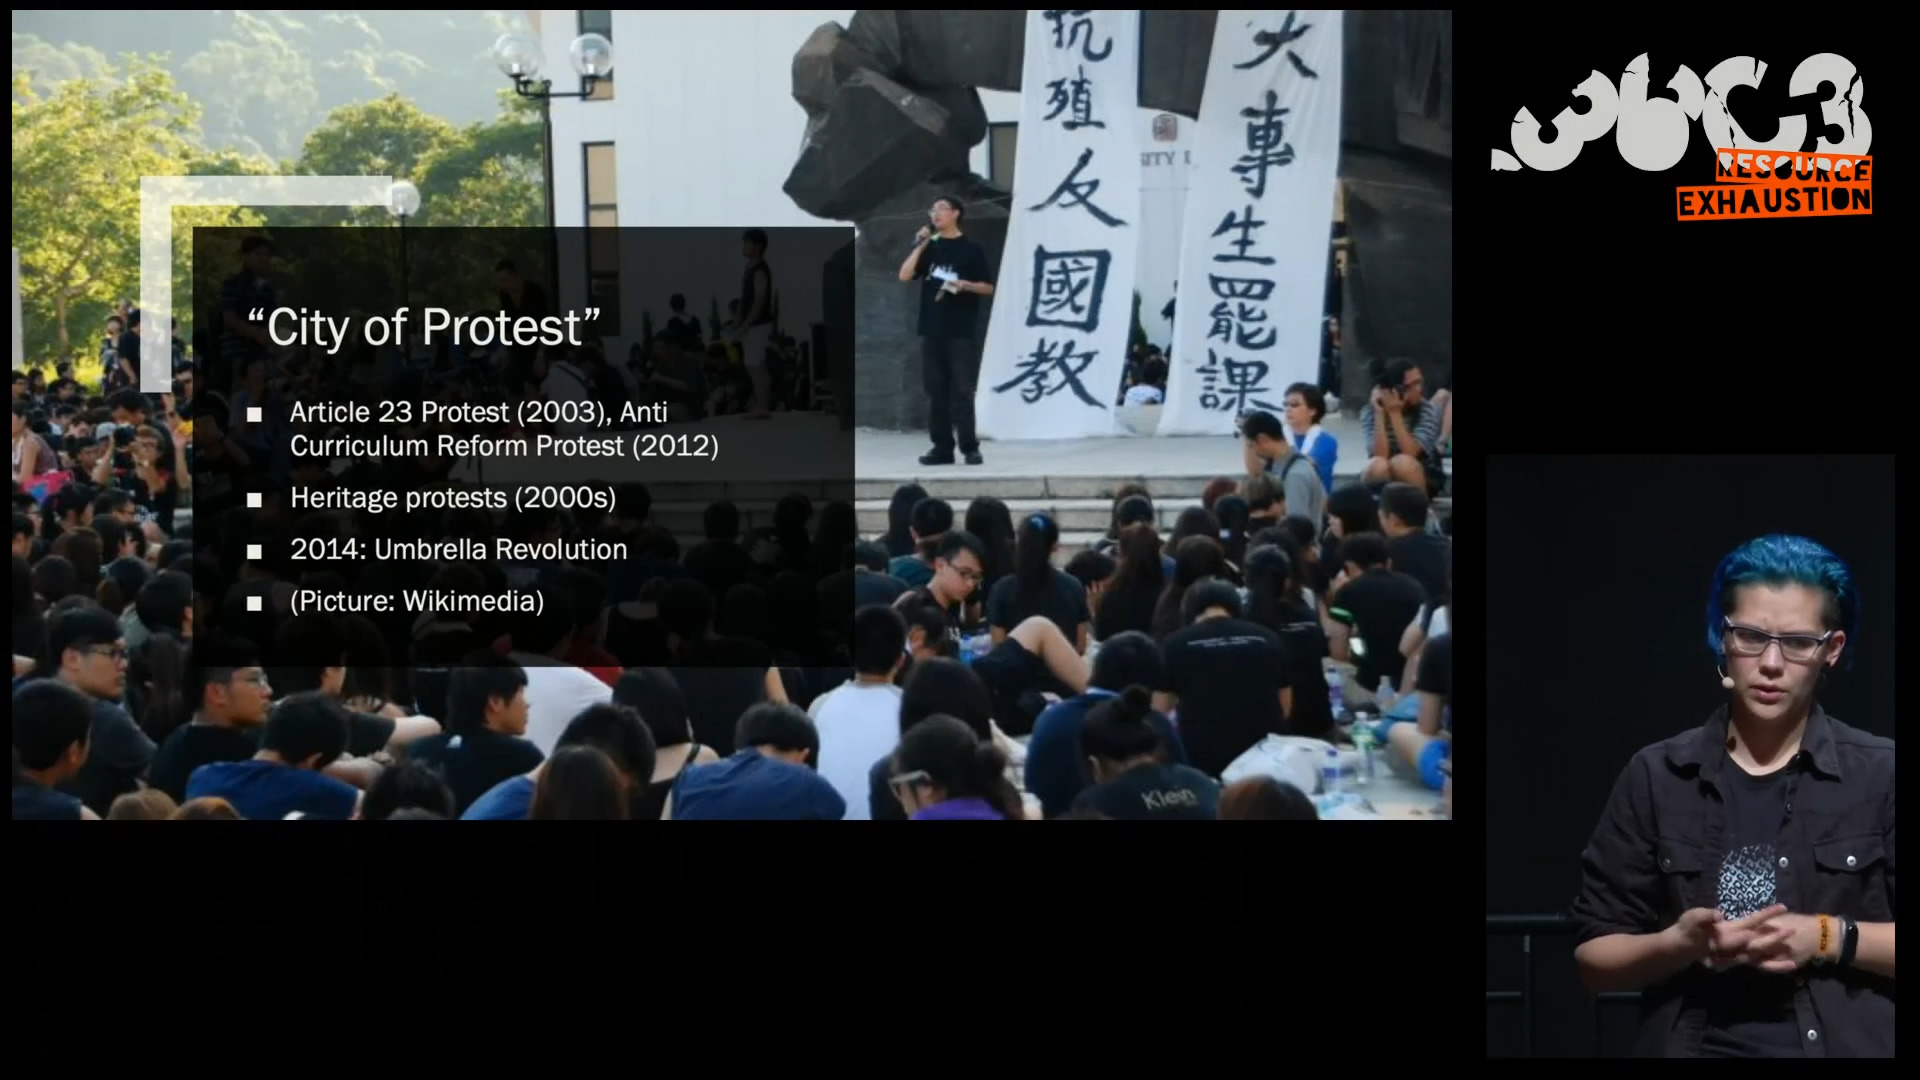
\includegraphics[width=0.75\textwidth]{images/shot-closeup2.jpg}
		\caption{Good closeup in Lecture Mode}
	\end{figure}
\end{frame}

\begin{frame}{Closeup Shot: Bad Example}
	\begin{figure}
		\centering
		
\includegraphics[width=0.75\textwidth]{images/shot-closeup-bad1.png}
		\caption{Half a head - not good}
	\end{figure}
\end{frame}

\begin{frame}{Closeup Shot: Bad Example}
	\begin{figure}
		\centering
		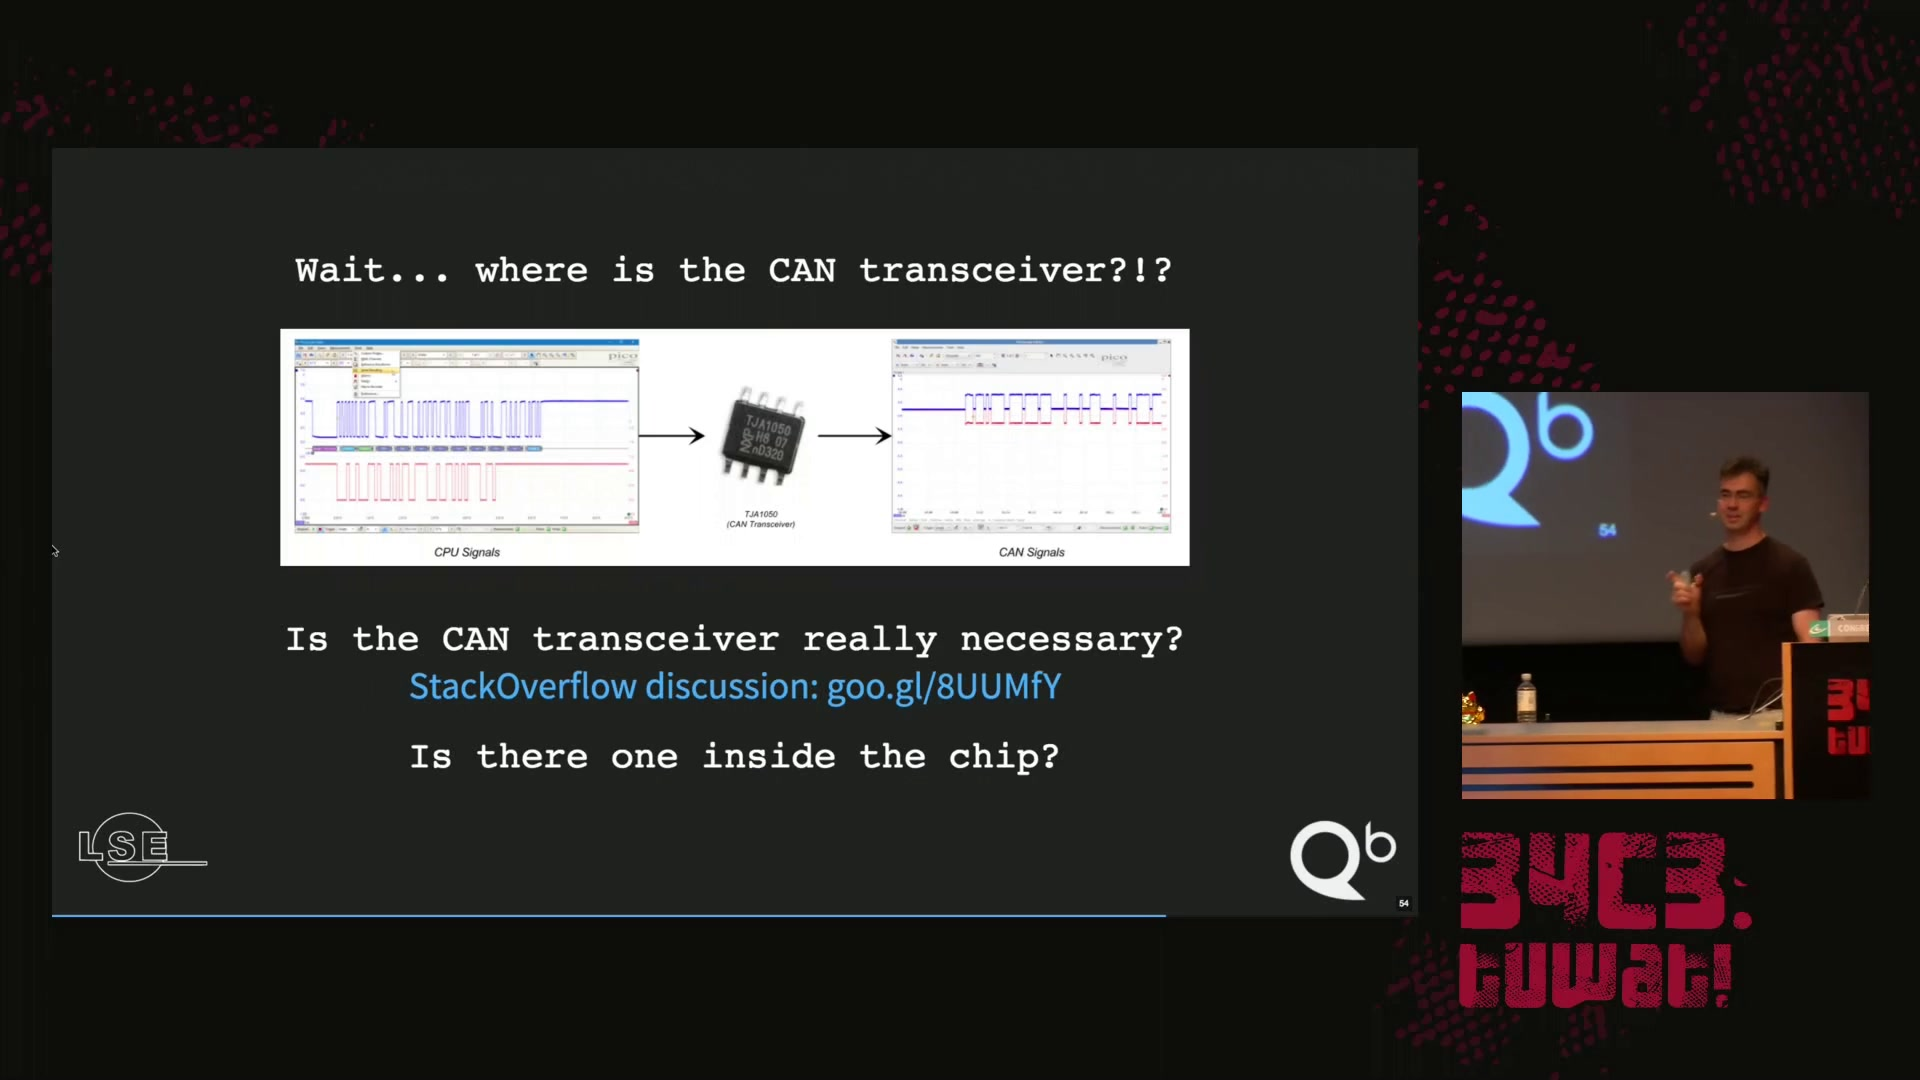
\includegraphics[width=0.75\textwidth]{images/shot-closeup-bad2.png}
		\caption{Too far out for a good Lecture Mode image}
	\end{figure}
\end{frame}

\begin{frame}{Medium Shot: Good 1}
	\begin{figure}
		\centering
		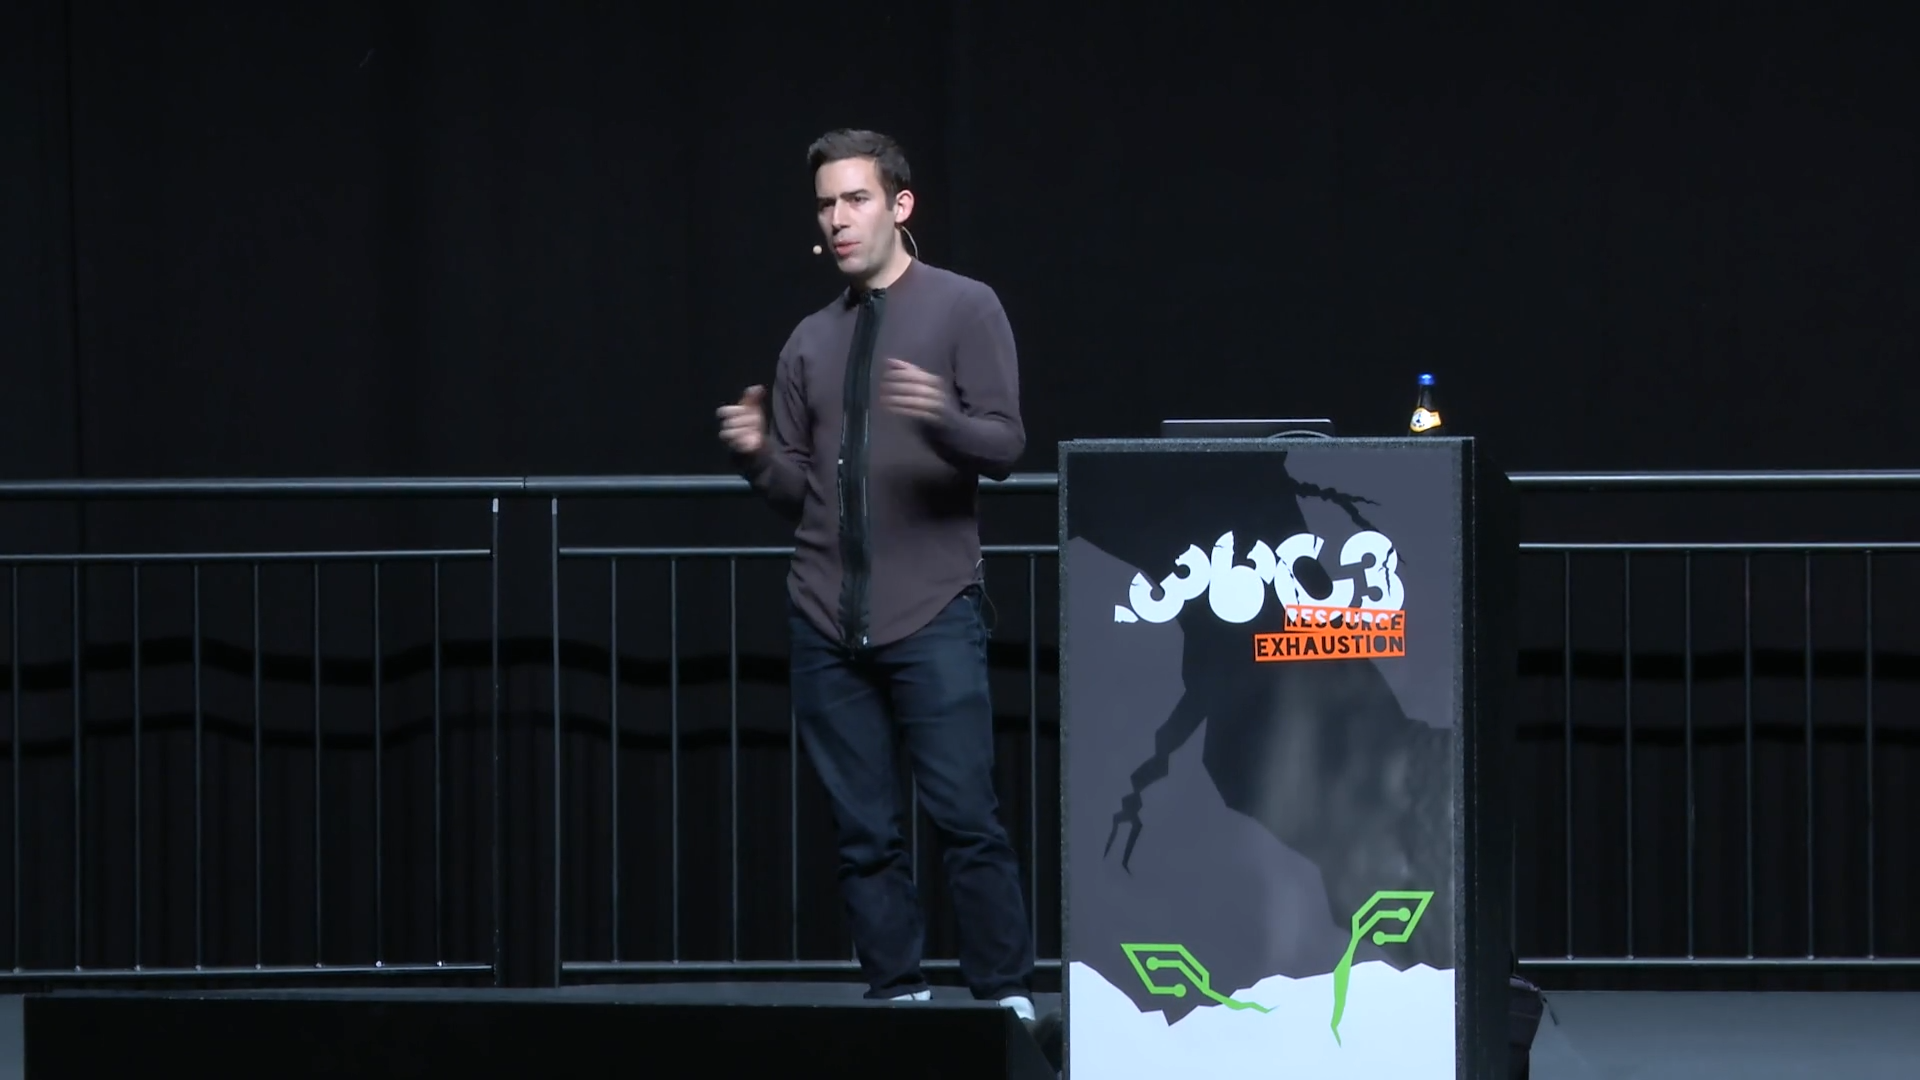
\includegraphics[width=0.75\textwidth]{images/shot-medium1.png}
		\caption{One person, the lectern and some context}
	\end{figure}
\end{frame}

\begin{frame}{Medium Shot: Good 2}
	\begin{figure}
		\centering
		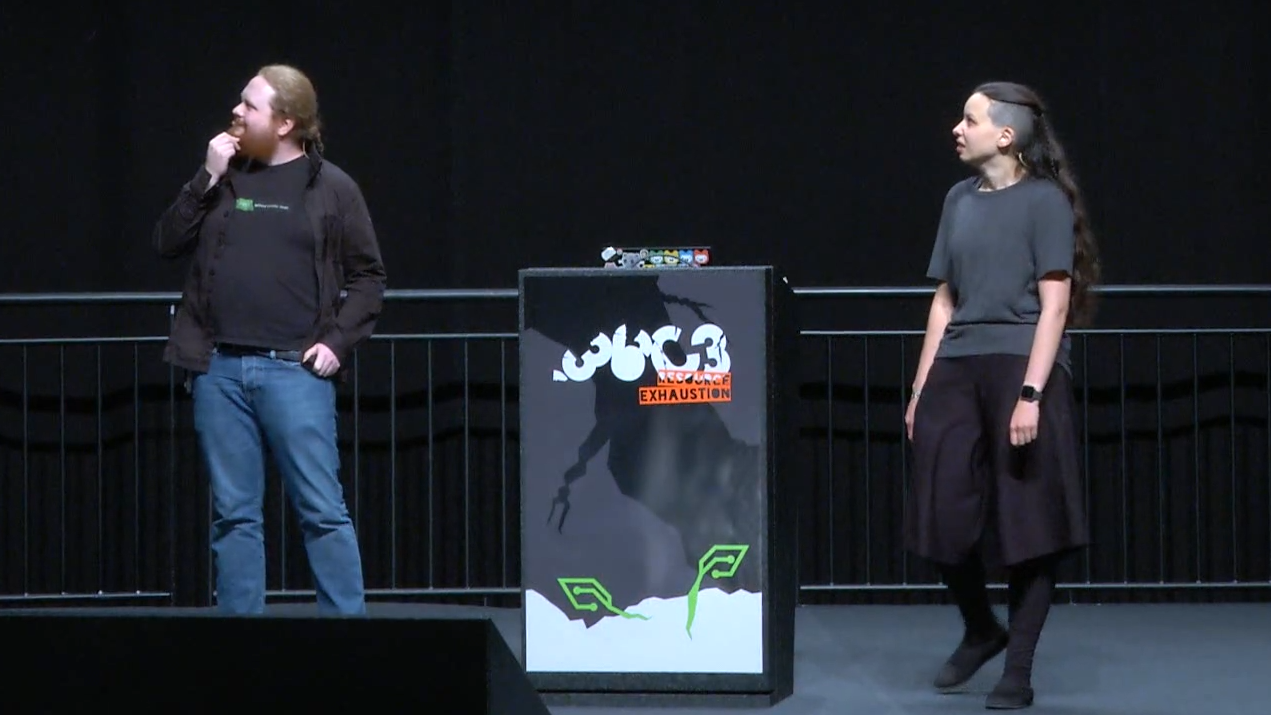
\includegraphics[width=0.75\textwidth]{images/shot-medium2.png}
		\caption{Two persons on stage}
	\end{figure}
\end{frame}

\begin{frame}{Overview}
	\begin{itemize}
		\item Shows the complete stage and the people on it
		\item Heads of the crowd are OK, if it's dark enough
		\item Don't use this camera to show the slides - use lecture mode instead
		\item Locked off, do not move.
	\end{itemize}
\end{frame}

\begin{frame}{Wide Shot: Good Example}
	\begin{figure}
		\centering
		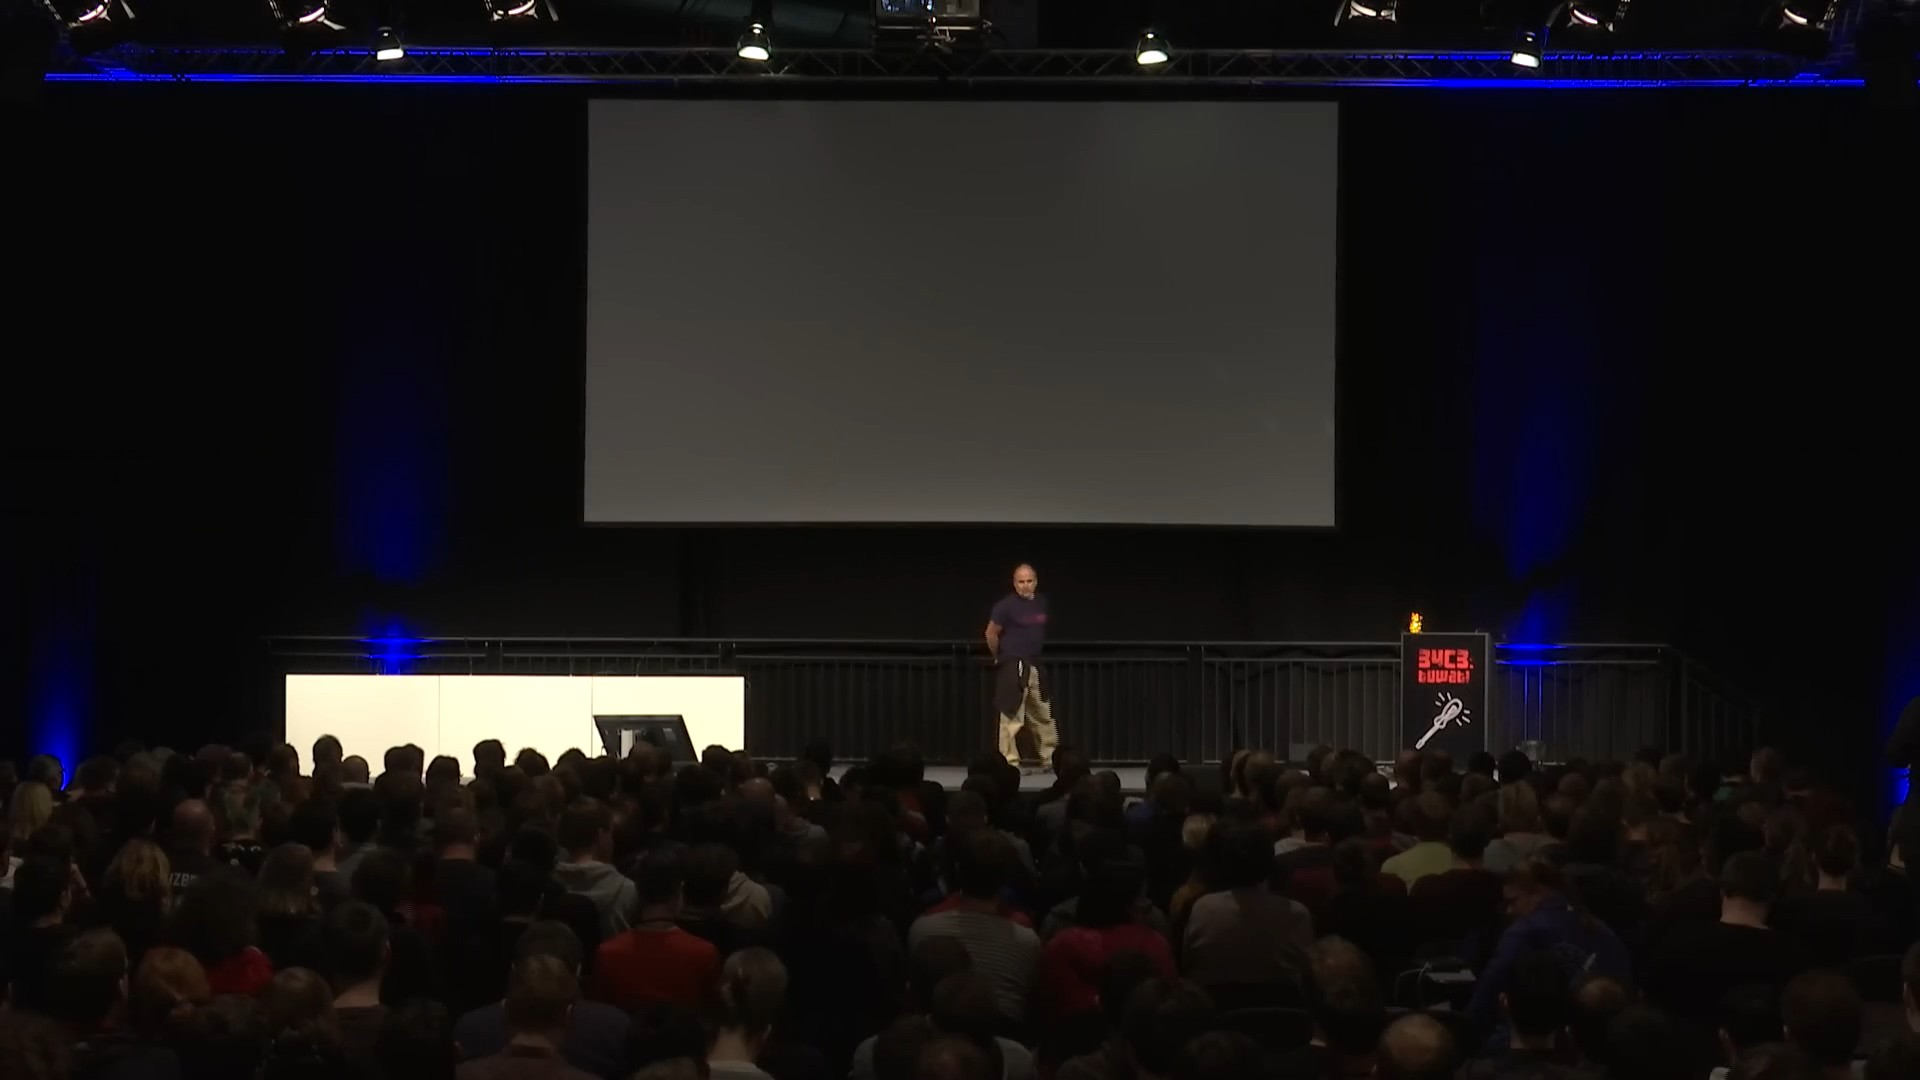
\includegraphics[width=0.75\textwidth]{images/shot-wide.jpeg}
	\end{figure}
\end{frame}


\end{document}
